\subsubsection{QuizziPedia::Back-End::App::Models}

\label{QuizziPedia::Back-End::App::Models}
\begin{figure}[ht]
	\centering
	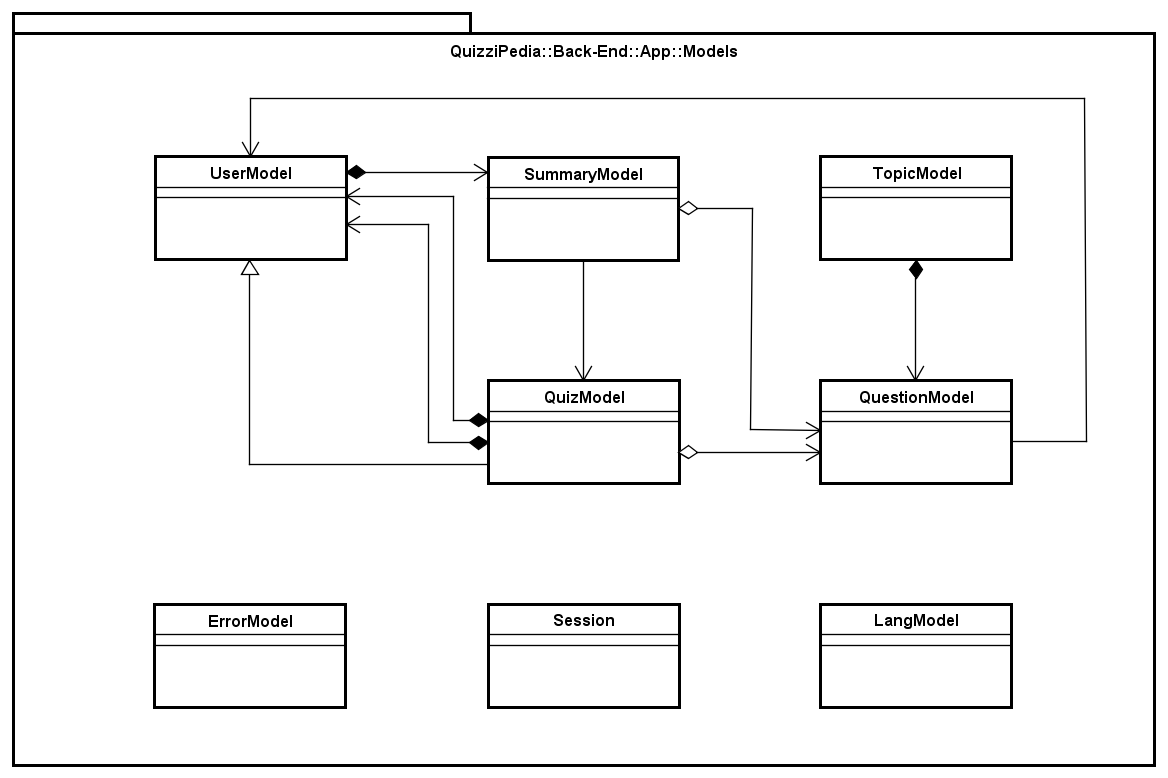
\includegraphics[scale=0.4]{UML/Package/QuizziPedia_Back-End_App_Models.png}
	\caption{QuizziPedia::Back-End::App::Models}
\end{figure}
\FloatBarrier
\begin{itemize}
	\item \textbf{Descrizione}: \textit{package\ped{G}} contenente le classi che definiscono il \textit{model} dell'applicazione. Queste classi sono definite come classi schema di \textit{Mongoose\ped{G}}, il quale permette di utilizzare \textit{MongoDB\ped{G}} tramite oggetti;
	\item \textbf{Padre} \texttt{App};
	\item \textbf{Interazioni con altri componenti}:
	\begin{itemize}
		\item \texttt{Controllers}:
		\textit{package\ped{G}} che contiene i \textit{controllers\ped{G}}  di \textit{Express\ped{G}}, definisce la logica dell'applicazione.
	\end{itemize}
	\item \textbf{Classi Contenute}:
	\begin{itemize}
		\item \texttt{Session}: classe che gestisce la sessione utente dell'applicazione. Non sono stati modellati attributi e metodi di questa classe in quanto viene inizializzata da \textit{Express\ped{G}} ed utilizzata da \textit{Passport\ped{G}} attraverso funzionalità interne ai due \textit{middleware\ped{G}};
		\item \texttt{UserModel}: classe che modella la creazione e la gestione dei dati utente;
		\item \texttt{UserProModel}: classe che modella i dati dell'utente pro;
		\item \texttt{QuestionModel}: classe che modella i dati relativi alle domande all'interno dell'applicazione;
		\item \texttt{QuizModel}: classe che modella i questionari all'interno dell'applicazione;
		\item \texttt{TopicModel}: classe che modella gli argomenti all'interno delle domande;
		\item \texttt{SummaryModel}: classe che modella i riepiloghi all'interno dell'applicazione;
		\item \texttt{LangModel}: classe che modella le informazioni riguardanti la lingua dell'applicazione;
		\item \texttt{ErrorModel}: classe che rappresenta le informazioni di un errore che si è verificato eseguendo una determinata operazione;
	\end{itemize}
\end{itemize}